
\documentclass[tikz,border=7pt]{standalone}
\usepackage[utf8]{inputenc}
\usepackage[T1]{fontenc}
\usepackage{amsmath}
\usepackage{xcolor}
\usetikzlibrary{arrows.meta,calc,angles,quotes,patterns,positioning}
\definecolor{brand}{HTML}{1E3A8A}
\definecolor{brandtwo}{HTML}{2563EB}
\definecolor{accentred}{HTML}{EF4444}
\definecolor{accentgreen}{HTML}{16A34A}
\definecolor{accentorange}{HTML}{F59E0B}
\definecolor{muted}{HTML}{64748B}
\definecolor{lightblue}{HTML}{EEF6FF}
\tikzset{force/.style={-{Latex[length=3mm]}, line width=1.15pt}, axis/.style={-{Latex[length=2mm]}, line width=.8pt, color=muted}, body/.style={draw=brandtwo, fill=lightblue, line width=1pt, rounded corners=2pt}, lab/.style={font=\small, text=brand}, sml/.style={font=\scriptsize, text=muted}}
\begin{document}

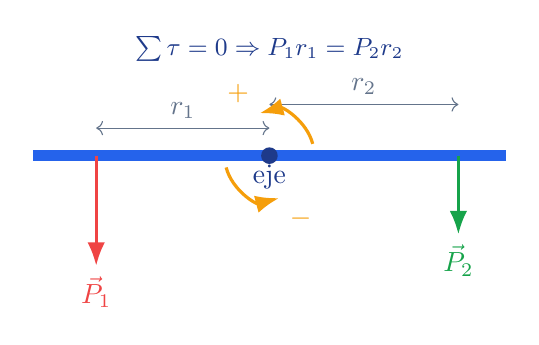
\begin{tikzpicture}[scale=1]
\draw[line width=4pt, color=brandtwo] (-3,0)--(3,0); \fill[brand] (0,0) circle (3pt) node[below] {eje};
\draw[force,color=accentred] (-2.2,0)--(-2.2,-1.4) node[below] {$\vec P_1$};
\draw[force,color=accentgreen] (2.4,0)--(2.4,-1) node[below] {$\vec P_2$};
\draw[<->,muted] (0,.35)--(-2.2,.35) node[midway,above] {$r_1$}; \draw[<->,muted] (0,.65)--(2.4,.65) node[midway,above] {$r_2$};
\draw[force,color=accentorange] (.55,.15) arc[start angle=15,end angle=105,radius=.55] node[above left] {$+$};
\draw[force,color=accentorange] (-.55,-.15) arc[start angle=195,end angle=285,radius=.55] node[below right] {$-$};
\node[lab] at (0,1.35) {$\sum\tau=0 \Rightarrow P_1r_1=P_2r_2$};
\end{tikzpicture}

\end{document}